\chapter{State-of-the-Art}

\section{Evolution of TA-definitions}

Several attempts were made to formally define the timing anomaly. Here we give a review of some definitions which can be applied to our architecture model.

\subsection{Step Heights}

Gebhard \cite{gebhard_timing_2012} gives a timing-anomaly definition based on local execution time of instruction in comparison to global execution time defined as sum of local ones. TA exists when local execution time of earlier instruction is lower and the global execution time of some later instruction is higher (compared to other trace).

Figure \ref{fig:step-good} shows this definition applied to example \ref{ex:simple-ta}. Orange arrow illustrates the local execution time of instruction $A$. The global time for instruction $D$ is different between traces $\alpha$ and $\beta$ (13 and 11 respectively).

\begin{figure}[!htb]
    \centering
    \begin{subfigure}[t]{0.5\textwidth}
        \centering
        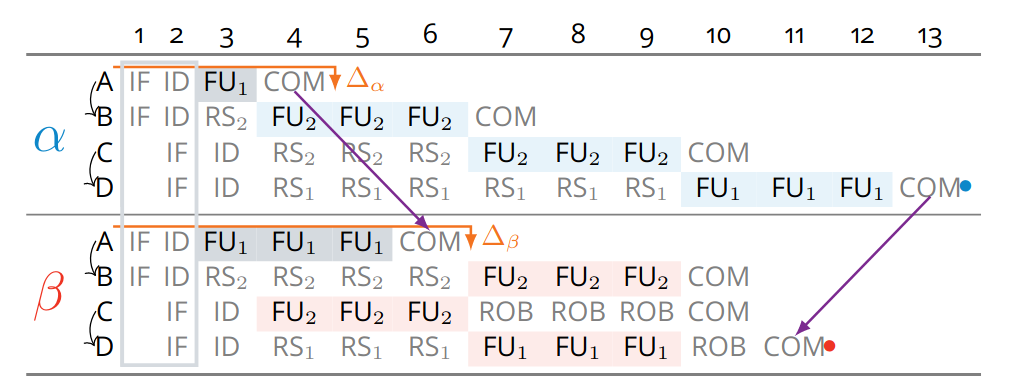
\includegraphics[width=\textwidth]{figures/step-func-good.png}
        \caption{Interpretation of example \ref{ex:simple-ta} using Gebhard's definition}
        \label{fig:step-good}
    \end{subfigure}
    \hfill
    \begin{subfigure}[t]{0.49\textwidth}
        \centering
        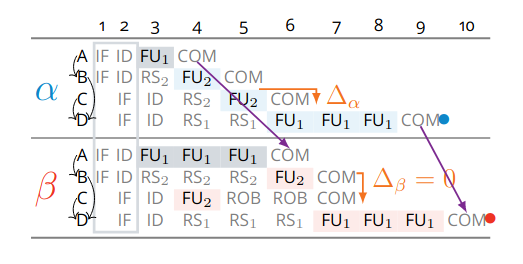
\includegraphics[width=\textwidth]{figures/step-func-bad.png}
        \caption{Counterexample to the definition}
        \label{fig:step-bad}
    \end{subfigure}
    \caption{Gebhard's definition applied to execution traces (from \cite{binder_definitions_2022})}
    \label{fig:step}
\end{figure}

In his thesis \cite{binder_definitions_2022}, Binder provides a counterexample (figure \ref{fig:step-bad}), where it is clear that there is no TA (trace $\beta$ has both unfavorable variation and longer execution time). However, the Gebhard's definition signals an anomaly because of shorter local execution time of instruction $C$ in trace $\beta$.

This poses a question whether it is reasonable to capture a local execution time as difference between instruction completion times. 

\subsection{Step-functions Intersections}

Similar definition is proposed by Cassez et al. \cite{cassez_what_2012}. The difference is that only global execution time is taken into account. Thus, TA arises when step-functions (that map instructions to their absolute completion time) of two traces intersect. 

\begin{figure}[!htb]
    \centering
    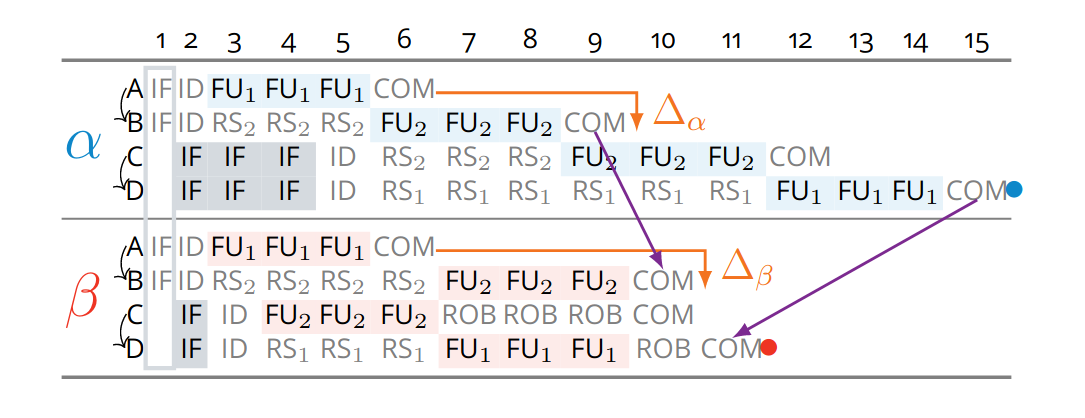
\includegraphics[width=\textwidth]{figures/step-func-2-bad.png}
    \caption{Contradicting result of Cassez's definition (from \cite{binder_definitions_2022})}
    \label{fig:step-2}
\end{figure}

This definition also leads to misleading effect with scenario found by Binder \cite{binder_definitions_2022}. Figure \ref{fig:step-2} iluustrates this by comparing two traces. Step-functions of traces $\alpha$ and $\beta$ intersect, however there is no counter-intuitive TA happening as $\alpha$ is both longer and hasa  longer latency for IF stage of instructions $C$ and $D$.

\subsection{Component Occupation}

An alternative approach is proposed by Kirner et al. \cite{kirner_precise_2009}. In their work the idea is to partition hardware into components and for each define the occupation by instruction (for how many cycles it processes the instruction). TA arises when a shorter component occupation coincides with a longer execution time in a chosen trace. However, as is shown is \cite{binder_definitions_2022} the results depend on how we define component partition which imposes the major concern against using this definition.

\TODO{counterexample}

\subsection{Instruction Locality}
\subsection{Progress-based definition}

Hahn and Reineke \cite{hahn_design_2020} intorduce the notion of progress, ... \cite{gruin_minotaur_2023}

\subsection{Event Time Dependency Graph}

Binder et al. \cite{binder_definitions_2022} define TAs using the notion of causality between events in execution trace. In this work, multiscalar OoO pipeline is considered. The processor state is described as a composition of states of each of the resource: \textit{IF, ID, set of RS, set of FU, ROB, COM}. Each component holds the information about instruction it is currently processing, including required registers and remaining clock cycles.

Notion of event is introduced based on qualitative changes in the pipeline associated to instruction progressing through stages. Event from execution trace (denoted as $e \in Events(\alpha$)) is a triple $(i,r,t)$, where $i$ is the instruction to which event is related, $r$ is the associated resource and the action (acquisition or release) and $t$ is a timestamp corresponding to the clock cycle when event occurs.

In the proposed framework events are related to \textit{IF, ID, FU} and \textit{COM} stages. For each instruction there are 7 types of events: $\IFa$, $\IFr$, $\IDa$, $\IDr$, $\FUa$, $\FUr$ and $COM$. $\uparrow$ signs the acquisition of a resource and $\downarrow$ its release. $COM$ denotes the acquisition of the commit stage, its release is not captured by the framework.

\textbf{Latency} is defined as a time difference between an acquisition of some resource and a release of it. For each pair of traces corresponding to the same program the sets of events are only different by the timestamps. Thus, for each event in one trace there is a corresponding event in the other one. Formally, it is a fucntion $CospEvent: Events(\alpha) \rightarrow Events(\beta)$.

A \textbf{variation} signs that the latency in one trace differs from latency of corresponding events in the other trace. On the pair of traces $\alpha$ and $\beta$. The variation is considered favorable for $\alpha$ if the latency in $\alpha$ is smaller than in $\beta$.

Variations are chosen as a source of timing anomalies. They may represent different memory behavior (cache hit or miss) for fetch and memory accesss in FU. Other sources of TA such as memory bus contention or branching are not considered by the framework.

\textbf{Event Time Dependency Graph (ETDG)} of trace $\tau$ denoted as $G(\tau) = (\mathcal{N}, \mathcal{A})$ is composed of a set of nodes $\mathcal{N} = Events(\tau)$ and a set of arcs $\mathcal{A} \subseteq \mathcal{N} \times \mathcal{N} \times \mathbb{N}$. 


Arc is a triple $(e_1, e_2, w)$ written as $e_1 \xrightarrow{w} e_2$ where $e_1$ is the source event node, $e_2$ -- destination node and $w$ is a lower bound of the delay between the two events. The arc means that at least $w$ clock cycles must pass between $e_1$ and $e_2$. 

Arcs are derived from a set of rules:
\begin{enumerate}
    \item \textbf{Order of pipeline stages}
    
    $(I, \IFa, t_0) \xrightarrow{lat_{IF}} (I, \IFr, t_1) \xrightarrow{0} (I, \IDa, t_2) \xrightarrow{1} (I, \IDr, t_3) \xrightarrow{0} (I, \FUa, t_4)  \xrightarrow{lat_{FU}} (I, \FUr, t_5)  \xrightarrow{0} (I, COM, t_6)$

    $lat_{IF}$ and $lat_{FU}$ are the latencies of IF and FU stages respectively.

    \item \textbf{Resource use}
    
    $lat_{IF} = t_1 - t_0$, $lat_{FU} = t_5 - t_4$

    \item \textbf{Instruction order}
    
    In-order part of the pipeline is constrained by instruction order. Thus, for successive instructions $I_1$ and $I_2$:

    $(I_1, RES\uparrow, t) \xrightarrow{0} (I_2, RES\uparrow, t'), RES \in \{IF, ID, COM\}$


    \item \textbf{Data dependencies}
    
    RAW dependency between $I_1$ and $I_2$ (\TODO{dep notation}) restricts the execution order of the instructions:  $(I_1, \FUr, t) \xrightarrow{0} (I_2, \FUa, t')$.
    
    \item \textbf{Resource contention}
    
    Also some instruction can be delayed because of limited resources. For instance, FU contention happens when $I_1$ and $I_2$ use the same FU, and it is busy by $I_1$ at the moment when $I_2$ is ready. This creates $(I_1, FUr, t) \xrightarrow{0} (I_2, FUa, t')$. 

    Resource contention can also be caused by reaching the capacity limit of ROB or RS. 
\end{enumerate}

\textbf{Causality graph} is achieved from ETDG by removing unnecessary edges. For each event we keep only the most relevant constraint. Only arcs of the form $e_1 \xrightarrow{e_2.time - e_1.time} e_2$ are left. Also arcs related to variations are excluded.

\textbf{Timing anomaly} is observed on pair of traces $\alpha$ and $\beta$ if there exists a favorable variation in $\alpha$ relative to $\beta$. Let $e_\alpha\downarrow$ and $e_\beta\downarrow$ be the events corresponding to the end of the variation in both traces. If there exist events $e_\alpha$ and $e_\beta$, where $e_\beta = CospEvent(e_\alpha)$ and there is a path in causality graph of $\alpha$ between $e_\alpha\downarrow$ and $e_\alpha$, s.t. $\Delta(e_\beta\downarrow,e_\beta) < \Delta(e_\alpha\downarrow,e_\alpha)$.


\begin{figure}[htbp]
    \centering
    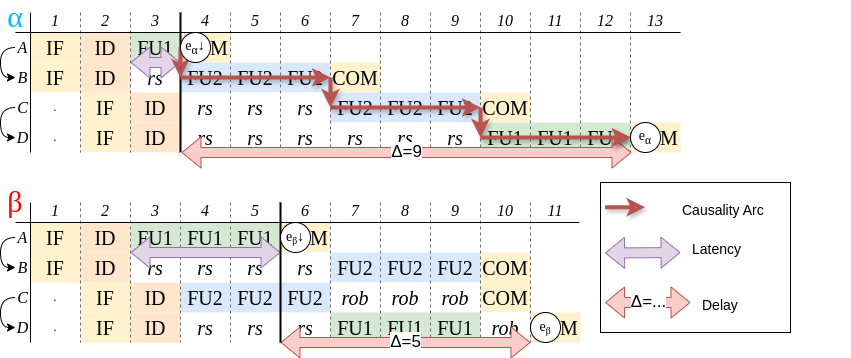
\includegraphics[width=0.8\textwidth]{figures/multiscalar_ta_causality.png}
    \caption{Causality-based TA detection applied for example \ref{ex:simple-ta}. $e_\alpha\downarrow = (A, \FUr, 4), e_\beta\downarrow = (A, \FUr, 6), e_\alpha = (A, COM, 13), e_\beta = (A, COM, 11)$. Purple arrow denotes latency which has a variation between two traces. Gray arrow shows delay between events which is greater in favorable trace. Causality in  path $\alpha$ is marked by red arrows.}
    \label{fig:multiscalar-ta-causality}
\end{figure}

\begin{figure}[htbp]
    \centering
    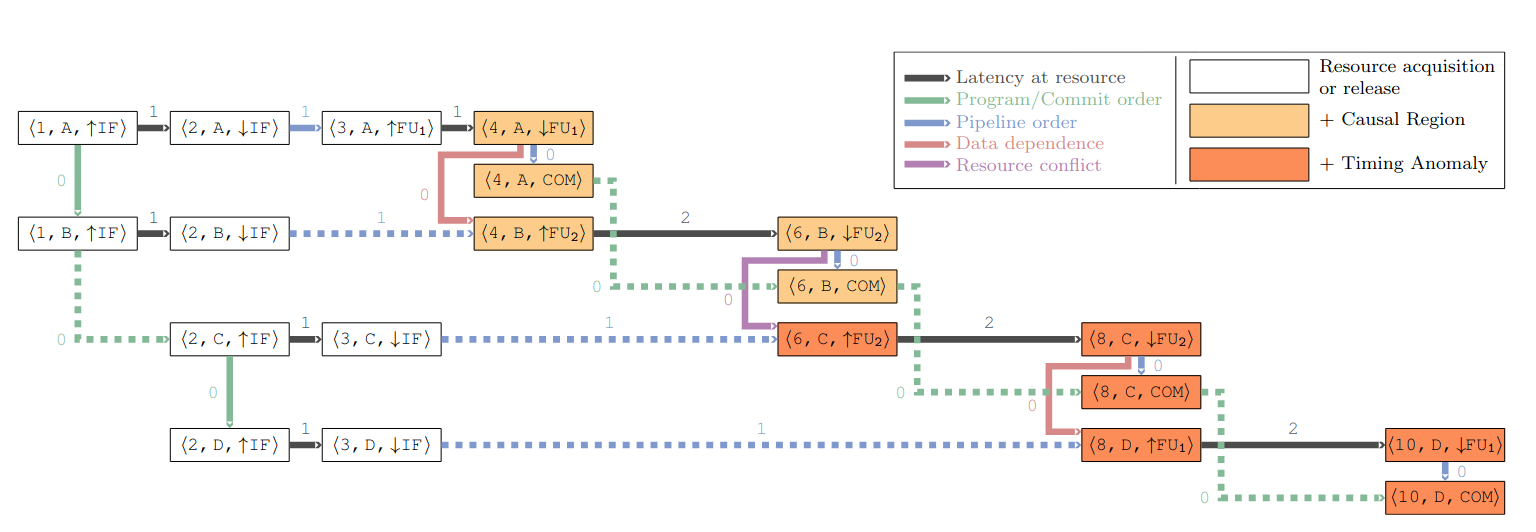
\includegraphics[width=\textwidth]{figures/ETDG.png}
    \caption{Complete ETDG for trace $\alpha$ from figure \ref{fig:multiscalar-ta}. \TODO{image source}}
    \label{fig:ETDG}
\end{figure}

Figure \ref{fig:multiscalar-ta-causality} shows how the framework captures TA for example \ref{ex:simple-ta}. Figure \ref{fig:ETDG} presents the complete ETDG for trace $\alpha$ with different dependency rules highlighted with different colors. The arcs reflecting causality are depicted in solid lines.

In contrast to other definition, this one measures relative time from the acquisition of the resource instead of global time. This approach allows the separation of different variations and isolates the part of the trace that experiences TA-effect.


\section{TA-classifications}

